\chapter{Approach}\label{chap:chap4}

\section*{}

This chapter describes the developed approach during the course of this
dissertation. First we describe its high level architecture, and then we move on
to describe each of the main phases that comprise it. For each phase, we
describe the phase both at a general level and its materialization (its main
goal, the most important variables, constraints, and methods). 

Finally, we describe the experimental setup of the approach, and the setup for
each component, and introduce the next chapter.

\section{High-level Architecture}

\begin{figure}[h] \begin{center} \leavevmode
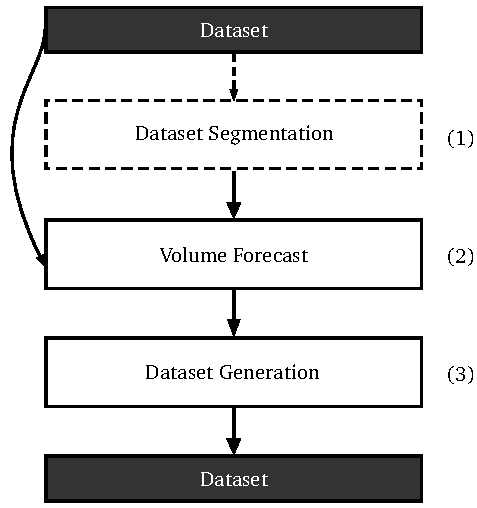
\includegraphics[]{high_level} \caption{ High level overview
of the approach } \label{fig:highlevel_arch} \end{center} \end{figure}

As the figure~\ref{fig:highlevel_arch} makes clear, the goal of the
proposed approach is to use a dataset containing logs of the web
activity from an online advertising related network and use this information 
to generate a possible future web activity logs on the same network. 
This should be done in order to preserve tendencies and into data coherency.

This approach can be divided into three main phases:
\begin{enumerate}
\item \emph{Segmentation},
which its main purpose is divide the dataset in smaller and more predictable
datasets, in order to improve the results obtained after the second phase, mostly when there
are large quantities of data available.

\item The second phase is where the \emph{forecast of the volumes} that characterize the traffic on
the network are done, using time series prediction methods.

\item The third and last phase of the process, the more complex one, is where the volumes
generated from the phase two combined with the data provided by the original
dataset are used to \emph{generate a dataset} that represent a possible future of the
web activity on the target network.
\end{enumerate}
\section{Architecture for Web Activity Forecasting and Synthesising}

\subsection{Data Segmentation}\label{subsec:seg}

\begin{figure}[h] \begin{center} \leavevmode
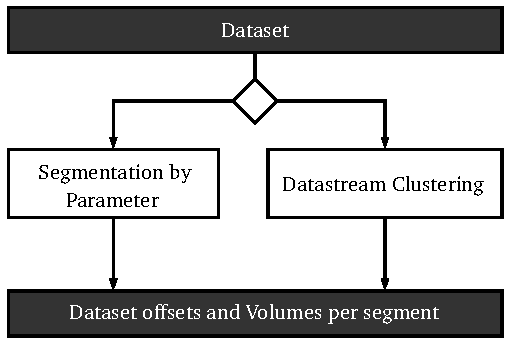
\includegraphics[]{segmentation} \caption{ High level overview
of Data Segmentation} \label{fig:segmentation_arch} \end{center} \end{figure}

The \emph{Data Segmentation} phase was designed in order to achieve better
results in the following phases. 

In order to get better results in the second phase (Volumes Forecast) the dataset needs to possess
certain characteristics that improve its predictability, or in other words, it
needs to have recurring trends and /or patterns.
One way of getting results is by splitting data by parameters known to have an
effect on traffic seasonality (for example the website that is being accessed).

As shown in figure~\ref{fig:segmentation_arch} the method described before was
one of the approaches chosen to achieve a more predictable time series.
This method allows clustering of the dataset via a selected parameter, which
returns \emph{impression clusters} in which all members of a cluster share the
same value in the parameter. This method requires great knowledge about the
available impressions to be successful.

The other approach that was implemented in this phase is a simplified and
striped down version of a \emph{data stream clustering} algorithm. This
algorithm is distance based, and since the structure of the datasets used on
this thesis are not guaranteed, the distance measure used is na\"{i}ve. The
distance between impressions can be described as:

\begin{center}
\begin{equation*}
  distance_{x,y}= \sum\limits_{i=0}^n d_i
\end{equation*}
\begin{equation*}
\text{where } d_i = \begin{cases} \text{1 if } x_i != y_x\\
\text{0 otherwise}\end{cases} \text{ and x, y are two impressions from the
dataset}
\end{equation*}
\end{center}

\begin{algorithm}
  \LinesNumbered
  \SetNlSty{texttt}{(}{)}
  \KwData{$lines$, all impressions available on the dataset; $threshold$,
  maximum distance to be considered member of a certain cluster.}
  \KwResult{A list of clusters, each one characterized by the $centroid$ and a list of
  offsets representing the position of each impression on the dataset.}
  \BlankLine

  \Repeat{no more impressions}{
    compare each impression with the existing list of clusters\;
    \eIf{ $dist < threshold$ }{
    add to the selected cluster\;
    }{create a new
    cluster and use the selected impression as the centroid for the new
    cluster\;}
  }
  \BlankLine

  \caption[Data stream clustering]{
    Data stream clustering simplified algorithm to aggregate the impressions by
    the parameters that they have in common.
  }
  \label{alg:pam} \end{algorithm}

This kind of algorithm was selected because, of the constraints imposed by the
problem, the most important ones are the huge volume of data this approach
needs to process, and the number and type of attributes that compose an
impression which may vary from dataset to dataset.

The huge volume of data invalidates the usage of
dissimilarity matrices due to memory constraints. The uncertainty of the
parameters that are available also limit the quality of the distance measure,
since it assumes that every parameter has the same weight as the others.

This family of clustering algorithms has some known limitations, for example, the
order in which the dataset is read directly influences the outcome of the
algorithm. There is also a problem with the centroids, since they are represented
by the attributes of the impression that originated that particular centroid,
and as such are never updated,
when a new impression has a distance lower than the threshold when compared with
a certain centroid, it is not assured that the respective cluster is the most
similar to the new impression.
In order to address this possible issue, the ability of calculate the distance
between the new impression and the available centroids and then select the one
with least distance was also implemented.

\subsection{Volume Forecasting}\label{subsec:volume_forecast}

\begin{figure}[h] \begin{center} \leavevmode
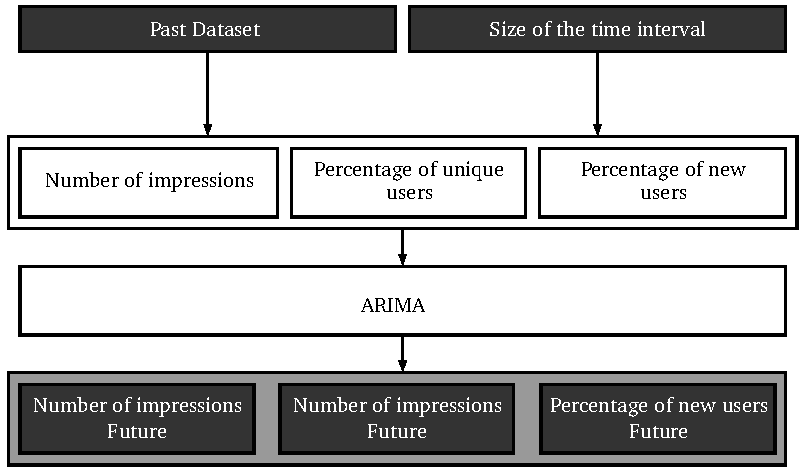
\includegraphics[]{forecast_volumes_arch} \caption{ High level overview
of Data Segmentation} \label{fig:forecast_volumes_arch} \end{center} \end{figure}

One way to describe the impressions is by representing how many happen during a
certain amount of time. So the impressions in the past can be described as time
series of volume of impressions, composed by uniformly spaced time intervals. 

So to predict how many impressions will happen in the future \emph{time series
analyses} techniques can be used. 

Since the volume of impressions doesn't allow to fully characterize the future
we need to use more time series of different variables which can provide more
 information about each epoch.

The approach here described involves the usage of three time series, one for the
number of impressions, other for the percentage unique users and a last one for
the percentage of unique users that had never appeared in the past.

\paragraph{Number of impressions}
is the number of entries on the dataset during each time interval.

\paragraph{Percentage of unique users}
is described by $\frac{\text{Number of users}}{\text{Number of impressions}}
* 100$, and represents how the number of users are related with the number of
impressions.

\paragraph{Percentage of new users}
represents per unit of time how many users that had never appeared before are
represented. It is described by $\frac{\text{Number of new users}}{\text{Number
of unique users}}*100$.
\\

So each unit of time can be represented by these three values. Now to
characterize the future, we need to forecast of these three values
on future time intervals. To complete this task the \emph{ARIMA} approach was
used separately for each of the three variables.


%******WHY DID I USED ARIMA

\subsection{Dataset Generator}

\begin{figure}[h] \begin{center} \leavevmode
\includegraphics[]{high_level_file_gen} \caption{ High level overview
of the Dataset Generator } \label{fig:highlevel_arch_file_gen} \end{center} \end{figure}

The last phase of the proposed approach generates a new dataset based on the
original dataset and the values of the three time series generated on the
previous phase (Volume Forecasting).

As shown in figure~\ref{fig:highlevel_arch_file_gen}, this phase was divided
into three sub-phases: the \emph{pre-process} (\ref{subsubsec:pre_process}), \emph{calculate
statistics} (\ref{subsubsec:stats}), and \emph{fill future data}
(\ref{subsubsec:fill_data}).

The pre-process sub-phase (\ref{subsubsec:pre_process}), breaks the old dataset
by interval size that was chosen on the volume forecasting phase
(\ref{subsec:volume_forecast}) and organizes the impressions per interval and
users.

The statistics calculation sub-phase, takes as input the processed data
from the past dataset and the volumes from the volume prediction phase
(\ref{subsec:volume_forecast}), verifies whether the values makes sense in the real
world, for example the number of impressions is higher than the number of users
(it is impossible for this type of dataset to have users with zero impressions,
since the dataset represents impressions), break the impressions into smaller
intervals, and use weekly historical data to predict the distribution of the
interval volumes on the smaller intervals.

The last sub-phase, fill future data (\ref{subsubsec:fill_data}), is the most
crucial phase of this process. It uses the volumes from the last sub-phase, and
then selects past impressions using the restrictions imposed by the calculated volumes. This
phase is also responsible for the generation of new users.

\subsubsection{Pre-process (i)}\label{subsubsec:pre_process}

\begin{figure}[h] \begin{center} \leavevmode
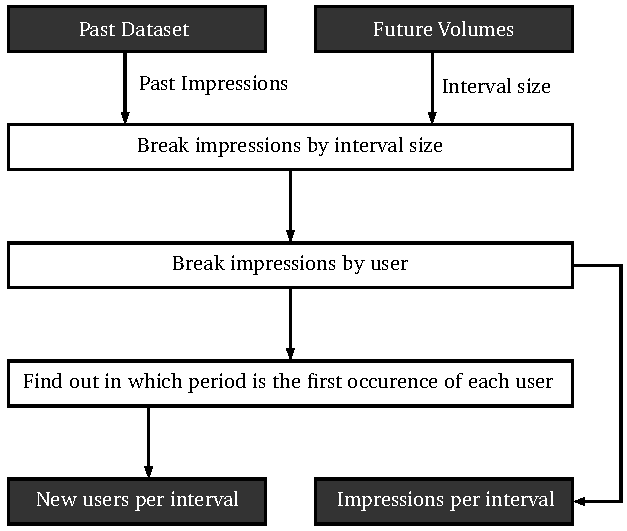
\includegraphics[]{pre_processing_i} \caption{ High level overview
of the Dataset Pre-processing} \label{fig:pre_processing_i} \end{center} \end{figure}

This phase (figure~\ref{fig:pre_processing_i}) can be considered the simpler phase of the whole approach. Its main
goal is to provide impressions organized by a defined time interval and 
place the first occurrence of each user in the correct interval, to better
organize data for the next phases.
\\

This is simply done by reading each line of the dataset and comparing with the
start date of the dataset placing it on the correct interval. It also identifies
which user is responsible for that impression and, if it is the first occurrence,
place it as a new user for the interval where the impression belong.

\subsubsection{Calculate Statistics (ii)}\label{subsubsec:stats}

\begin{figure}[h] \begin{center} \leavevmode
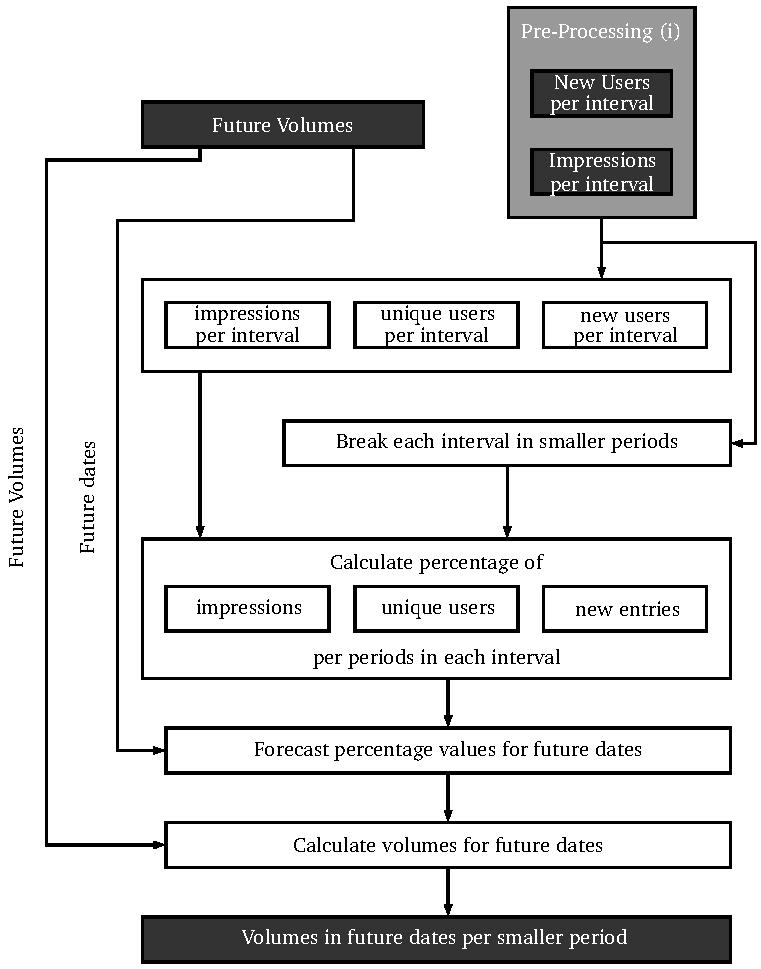
\includegraphics[]{calculate_stats} \caption{ High level overview
of statistics calculation} \label{fig:calculate_stats_ii} \end{center} \end{figure}

The main purpose of the sub-phase represented in the figure~\ref{fig:calculate_stats_ii} is
to distribute the volumes predicted for a certain interval in smaller periods
based on the historical distribution of the volumes for the same period.

In order to obtain better resolution of how the data is distributed on the
interval, these intervals are broken down in periods of one hour each. Now to
understand how the volumes of the interval are distributed through the time periods,
the data from the same interval up to two weeks before the interval which is
currently
being processed is used. For each hour period of historical interval the
percentage of the total volume is calculated.
To calculate the distribution , the input is the mean of the values from the
same interval, the week before, and two weeks before. If there is only one
previous week available, then the value of the current period is the same as the
value from the week before; if there are no previous weeks available, the
distribution of the interval volumes is done by dividing uniformly by each hour
period.
After the percentages are
calculated, they are multiplied by the total volumes to obtain the absolute
values for each interval.
\\
For each hour period the following values are calculated:
\begin{itemize}
  \item \textbf{Number of impressions}, this value represents how many requests
    were done during that space in time;
  \item \textbf{Number of users}, number of different users present during that
    space in time;
  \item \textbf{Number of first occurence users}, number of different users that
    occur for the first time in the interval during that specific hour period;
  \item \textbf{Number of new users}, number of different users that are
    completely new to the dataset and that occur for the first time in that specific
    hour period.
\end{itemize}

In order to be valid, these variables have to respect these constraints:
\begin{itemize}
\item the number of impressions must be equal or greater than the number of
  users for a specific period;
\item the number of users must be less or equal to the sum of number of first
  occurrence users;
\item the number of new users and number of users that appear on the one hour
periods prior to this period that belong to the same interval;
\item the number of first occurrence users plus the number of new users must be
  equal or less than the number of users for the time period.
\end{itemize}

To guarantee the integrity of the result, these conditions have to be verified.
So, after the calculation of the results for every hour period of a certain
interval of time, a constraint check is performed and the results
are adjusted accordingly.
And to do so the approach implemented according to
algorithm~\ref{alg:adjust_values} can be used to fulfil this task.
\\

\begin{algorithm}[H]
  \LinesNumbered
  \SetNlSty{texttt}{(}{)}
  \KwData{$periods$, a list of one tuple for each period; $volumes$,
  a tuple containing the expected values for the interval}
  \KwResult{A list of one tuple for each period, containing the adjusted values
  to meet the imposed constraints}
  \BlankLine

  \While{the sum tuples for all periods != $volumes$}{
    $diff$ = $volumes$ - $sum(periods)$\;
    \For{each element of $periods$}{
      To each constraint not respected, change the value according to the rule and
      then add the difference to the respective $diff$\;
      \If{any constraint not violated and the respective value of $diff$ is not
      0}{ 
        change the respective value while still respect the imposed constraint\;
      }
    }
}
  \BlankLine
  \vspace{0.5cm}
  \caption[Constraint adjustement for statistics]{
    Values adjustment to meet the imposed constraints algorithm
  }
  \label{alg:adjust_values} \end{algorithm}

At the end of this phase we have calculated all the four
values for every future interval for which we want to predict the impressions.


\subsubsection{Fill Future Data (iii)}\label{subsubsec:fill_data}

\begin{figure}[h] \begin{center} \leavevmode
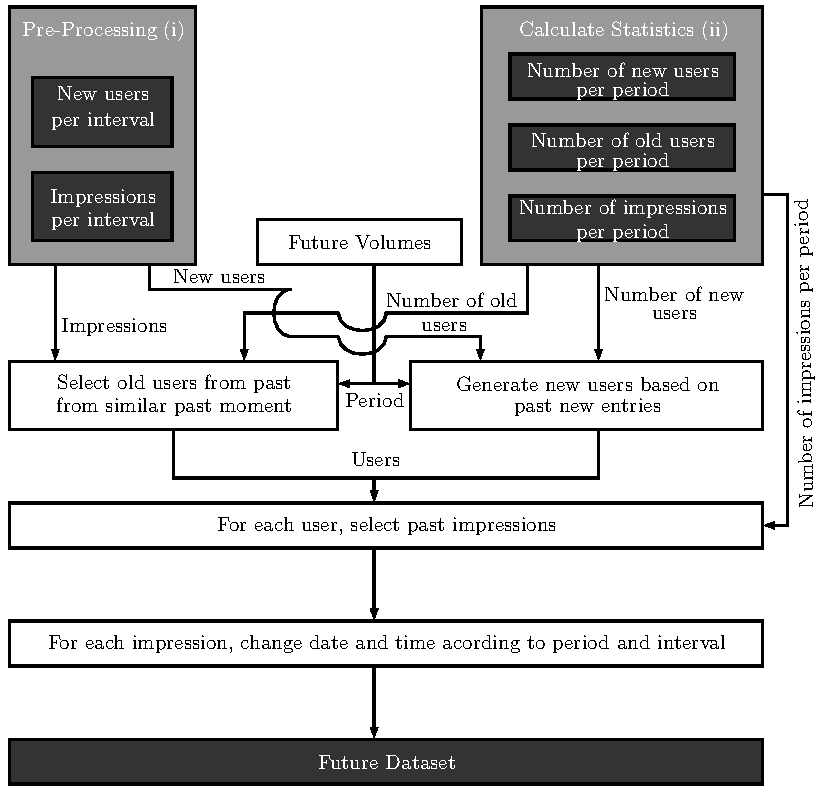
\includegraphics[]{fill_future} \caption{ High level overview
of fill future data} \label{fig:fill_future_iii} \end{center} \end{figure}

The last sub-phase of the dataset generation phase is responsible for selecting
which users and impressions, from the dataset that represents past activity,
will reappear in the future with some changes.

To be able to capture the correct characteristics, so that the future follows the
trends of the past, the first step must be the selection of the relevant periods of
time in the past that are equivalent to the one which is currently being filled.
This approach uses the same period from previous weeks ranked by proximity to
the date, which makes more likely to use users from the previous week than two
weeks ago.

After the correct dates are found, the users that will reappear in a given
period must be selected taking into account the limits imposed by the volumes
predicted on the previous sub-phase (\ref{subsubsec:stats}).

The process of the selection of old users is non-deterministic (uses random generated
values to select which past users will reappear), but assures that does not enter
an infinite loop, by terminating if it spends more than a $threshold$ of cycles
without getting a valid result. This is done in reverse chronological order,
where we first select users from the week before. If there are not enough
users we use data from previous weeks.

To complete the process of selection of users that will appear in the given
period, we need to ''generate'' new users. Since we have no knowledge of the
data that represents an impression other than it has a date and an user
identification token, this process is more a selection, than a generation, of
past users that occurred for the first time on similar periods of the past, and
then their date and user identification are changed according to the period for
where this user will reappear. Like the previous selection process, this one also
takes into account the chronological distance between events. First we use new
occurrences from the same period, starting on the previous week until the first date
of the past dataset (if there are not enough users available, users from the
same interval\footnote{Note that an interval is composed by multiple one hour
periods.} are used, if more users are needed then users from any interval of the
dataset are used)(Algorithm~\ref{alg:user_selection}).
\\

\begin{algorithm}[!htb]
  \LinesNumbered
  \SetNlSty{texttt}{(}{)}
  \KwData{
        \textbf{users\_period}, a list of lists of users reverse chronologically
    ordered\;\\
    \textbf{users\_from\_same\_interval},
  list of lists of users from the same interval as the one to be filled, also in
  reverse chronological order\;\\
  \textbf{all\_users}, list of all users from the past\;\\
  \textbf{period}, date and time interval which the new users will be part of\;
  \textbf{target\_new\_users}, number of new users\;
  }
  \KwResult{A list of new users, containing the impressions with user
    identification token, modified and timestamp,
    adjusted to the given period.}
  \BlankLine

  \emph{selected\_users} is initialized as an empty list\;

  \For{each \emph{date} in the past, in reverse chronological order}{
    \eIf{length of \emph{selected\_users} less than \emph{target\_new\_users}}{
    Randomly select users from \emph{users\_period} for the \emph{date} that are not in \emph{selected\_users}, until there
      are no more users or the \emph{target\_new\_users} is reached\;
    }{
      break\;
    }
  }
  \BlankLine

  \If{length of \emph{selected\_users} less than \emph{target\_new\_users}}{
  \For{each \emph{date} in the past, in reverse chronological order}{
    \eIf{length of \emph{selected\_users} less than \emph{target\_new\_users}}{
      Randomly select users from \emph{users\_from\_same\_interval} for \emph{date} that are not in \emph{selected\_users}, until there
      are no more users or the \emph{target\_new\_users} is reached\;
    }{
      break\;
    }
}}
  \BlankLine

  \If{length of \emph{selected\_users} less than \emph{target\_new\_users}}{
  \For{each \emph{date} in the past, in reverse chronological order}{
    \eIf{length of \emph{selected\_users} less than \emph{target\_new\_users}}{
      Randomly select users from \emph{all\_users} for \emph{date} that are not in \emph{selected\_users}, until there
      are no more users or the \emph{target\_new\_users} is reached\;
    }{
      break\;
    }
}}
\BlankLine
For all \emph{selected\_users} replaces the UUID and timestamp with a randomly
generated ones (timestamp belongs to given \emph{period})\;
  \BlankLine
  \vspace{0.5cm}
  \caption[User Generation Process]{
    User ''generation'' process.
  }
  \label{alg:user_selection}
\end{algorithm}


To complete the process of filling the future impressions, we still need to
select which past impressions from the selected users will be used, and modify
them according to the period that is being computed. First we randomly
select one impression from each user, since all the selected users must appear at
least one time. Afterwards, all the impressions are sorted in a random order, and
the impressions are selected randomly one by one until the requirements are
fulfilled.
The selection process takes into account the number of impressions associated
with a user; a user with many impressions in the past has more chances for one
of his impressions to be selected.
After all impressions are selected, their time value are updated to a random time
inside the current time interval.

These steps must be executed for each period that we want to predict.

At the end we have a complete dataset that represent the volumes predicted on
the Volume Forecasting phase (\ref{subsec:volume_forecast}), which are ready to be used on a simulator.

\section{Experimental Setup}

\subsection{Dataset format}

To develop this approach a dataset containing the time of the occurrence, user
id token, and other information, like the browser, location, cookies, etc. was
used, an example of this dataset in on the table~\ref{tab:dataset}.

\begin{table}[h]
\tiny
\begin{tabular}{lllll}
\multicolumn{1}{l|}{\textbf{Time}}                    & \multicolumn{1}{l|}{\textbf{UserId}}                      & \multicolumn{1}{l|}{\textbf{AdvertiserId}}     & \multicolumn{1}{l|}{\textbf{OrderId}}  & \textbf{LineItemId}         \\ \hline
\multicolumn{1}{l|}{2013-11-26-00:00:01}              & \multicolumn{1}{l|}{89e3b953-4422-49cb-bc10-8e869b30f0ab} & \multicolumn{1}{l|}{26621901}                  & \multicolumn{1}{l|}{138907941}         & 107293701                   \\
                                                      &                                                           &                                                &                                        &                             \\
\multicolumn{1}{l|}{\textbf{CreativeId}}              & \multicolumn{1}{l|}{\textbf{CreativeVersion}}             & \multicolumn{1}{l|}{\textbf{CreativeSize}}     & \multicolumn{1}{l|}{\textbf{AdUnitId}} & \textbf{CustomTargeting}    \\ \hline
\multicolumn{1}{l|}{32278541781}                      & \multicolumn{1}{l|}{1}                                    & \multicolumn{1}{l|}{1x2}                       & \multicolumn{1}{l|}{27191421}          & pos=0;showroom=ab           \\
                                                      &                                                           &                                                &                                        &                             \\
\multicolumn{1}{l|}{\textbf{Domain}}                  & \multicolumn{1}{l|}{\textbf{CountryId}}                   & \multicolumn{1}{l|}{\textbf{Country}}          & \multicolumn{1}{l|}{\textbf{RegionId}} & \textbf{Region}             \\ \hline
\multicolumn{1}{l|}{2e07dc054c5bdcec109605689ec8e11f} & \multicolumn{1}{l|}{2276}                                 & \multicolumn{1}{l|}{Germany}                   & \multicolumn{1}{l|}{20240}             & Saxony-Anhalt               \\
                                                      &                                                           &                                                &                                        &                             \\
\multicolumn{1}{l|}{\textbf{CityId}}                  & \multicolumn{1}{l|}{\textbf{City}}                        & \multicolumn{1}{l|}{\textbf{BrowserId}}        & \multicolumn{1}{l|}{\textbf{Browser}}  & \textbf{OSId}               \\ \hline
\multicolumn{1}{l|}{1004957}                          & \multicolumn{1}{l|}{Hettstedt}                            & \multicolumn{1}{l|}{500072}                    & \multicolumn{1}{l|}{Google Chrome}     & 501011                      \\
                                                      &                                                           &                                                &                                        &                             \\
\multicolumn{1}{l|}{\textbf{OS}}                      & \multicolumn{1}{l|}{\textbf{OSVersion}}                   & \multicolumn{1}{l|}{\textbf{BandWidth}}        & \multicolumn{1}{l|}{\textbf{TimeUsec}} & \textbf{AudienceSegmentIds} \\ \hline
\multicolumn{1}{l|}{Microsoft Windows 7}              & \multicolumn{1}{l|}{}                                     & \multicolumn{1}{l|}{adsl-8mbps}                & \multicolumn{1}{l|}{1384817822}        &                             \\
                                                      &                                                           &                                                &                                        &                             \\
\multicolumn{1}{l|}{\textbf{Product}}                 & \multicolumn{1}{l|}{\textbf{RequestedAdUnitSizes}}        & \multicolumn{1}{l|}{\textbf{BandwidthGroupId}} &                                        &                             \\ \cline{1-3}
\multicolumn{1}{l|}{Ad Server}                        & \multicolumn{1}{l|}{1x2}                                  & \multicolumn{1}{l|}{3}                         &                                        &                            
\end{tabular}
\caption{Example data from the dataset used with the respective label}\label{tab:dataset}
\end{table}

The only fields that the solution depends on are the time and the user id token,
all the other fields are optional and the approach described above does not have
any specific knowledge about them, nor it depends on it. The optional parameters
can be useful on the segmentation phase, to divide the dataset into smaller
datasets in order to capture more specific characteristics.

The design decision of not using anything besides the time and user id, was made
because the proposed solution should be agnostic of the data that it analyses.
Mostly because the data available is not standardised, and the solution should be
able to be used on data from multiple sources, with each source having its own
way of saving activities.

\subsection{Experimental Setup configurations}

In order to be able to test the previously described approach, the proposed
approach was implemented using $Python$. The experimental setup is completely
modular, with every phase being totally independent of the other. In other
words, any phase can use as input data from other sources other than the implemented
ones. Other than $Python$, $R$ was used in order to use the $ARIMA$ model.

\subsubsection*{Segmentation}

In this phase there are two implement methods, as explained
before in section~\ref{subsec:seg}. The $data stream-based$ algorithm has a
single configuration parameter, the threshold for the distance between the
impression that defines the clusters and the one that is being tested.
In the case of segmentation by parameters, the parameters to be used for
the division can be changed, so different configurations were tested.

This phase cannot be directly validated nor compared, so the results were
only validated and compared after the forecast phase.

The baseline method for this phase, divides the impressions on a chronological
order into 100 groups.

\subsubsection*{Volume Forecast}

On this phase, the $ARIMA$ model is used to predict the behaviour of the time
series for the time interval where we want to predict the volume values. To use
the $ARIMA$ model, the function $auto.arima$ from the package $forecast$
\cite{hyndman2007automatic} (from $R$)
was used, using a $Python$ wrapper in order to process the data. The $R$ is only
responsible for the prediction.

The function used allows the configuration of various parameters, most of which
were covered by the tests (for example, the usage of \emph{drift terms}).
The frequency of the time series object in
$R$ is also configurable.

Different time intervals were also tested, in order to understand which interval
produces better results.

To compare these results, $RMSE$ and $MASE$ where used.

The baseline method for this phase, copies data from the furthest date of the
dataset into the starting date of the forecast, respecting the day of the week
and the hour.

\subsubsection*{Dataset Generation}

This last phase does not take any additional parameters. It uses the values
that had been forecast in the volume forecast phase and the old dataset in order to build
a dataset which represents the future.

This phase was tested using synthetic generated past datasets which contained certain
changes in some parameters (examples: changes in browser usage and addition
of new domains).

Since a simulator was not available during the test phase, some queries over the
data were done to test the capability of this phase.

\section{Conclusion}

As mentioned before, this process has multiple phases where it tries to capture the
maximum amount of information about the past in order to more accurately predict
the future.
This chapter ends with an high level overview of the experimental setup, for which
the results will be presented and analysed on the next chapter.

